\documentclass{beamer}
\usepackage[utf8]{inputenc}

\usetheme{Madrid}
\usecolortheme{default}
\usepackage{amsmath,amssymb,amsfonts,amsthm}
\usepackage{txfonts}
\usepackage{tkz-euclide}
\usepackage{listings}
\usepackage{adjustbox}
\usepackage{array}
\usepackage{tabularx}
\usepackage{gvv}
\usepackage{lmodern}
\usepackage{circuitikz}
\usepackage{tikz}
\usepackage{graphicx}

\setbeamertemplate{page number in head/foot}[totalframenumber]

\usepackage{tcolorbox}
\tcbuselibrary{minted,breakable,xparse,skins}



\definecolor{bg}{gray}{0.95}
\DeclareTCBListing{mintedbox}{O{}m!O{}}{%
  breakable=true,
  listing engine=minted,
  listing only,
  minted language=#2,
  minted style=default,
  minted options={%
    linenos,
    gobble=0,
    breaklines=true,
    breakafter=,,
    fontsize=\small,
    numbersep=8pt,
    #1},
  boxsep=0pt,
  left skip=0pt,
  right skip=0pt,
  left=25pt,
  right=0pt,
  top=3pt,
  bottom=3pt,
  arc=5pt,
  leftrule=0pt,
  rightrule=0pt,
  bottomrule=2pt,
  toprule=2pt,
  colback=bg,
  colframe=orange!70,
  enhanced,
  overlay={%
    \begin{tcbclipinterior}
    \fill[orange!20!white] (frame.south west) rectangle ([xshift=20pt]frame.north west);
    \end{tcbclipinterior}},
  #3,
}
\lstset{
    language=C,
    basicstyle=\ttfamily\small,
    keywordstyle=\color{blue},
    stringstyle=\color{orange},
    commentstyle=\color{green!60!black},
    numbers=left,
    numberstyle=\tiny\color{gray},
    breaklines=true,
    showstringspaces=false,
}
%------------------------------------------------------------
%This block of code defines the information to appear in the
%Title page
\title %optional
{1.5.27}
%\subtitle{A short story}

\author % (optional)
{Manupati Manideep-EE25BTECH11039}




\begin{document}


\frame{\titlepage}
% Frame 1: Question
\begin{frame}{Question}
\begin{block}{Problem}
If the coordinates of points $\vec{A}$ and $\vec{B}$ are $(-2,2)$ and $(2,-4)$ respectively, find the coordinates of $\vec{P}$ such that
\[
AP = \frac{3}{7} AB.
\]
and $\vec{P}$ lies on line segment AB.

\end{block}
\end{frame}

% Frame 2: Process / Solution Steps
\begin{frame}{Solution Process}
\textbf{Given:}
\[
\vec{A} = \begin{bmatrix}-2 \\ 2\end{bmatrix},\qquad 
\vec{B} = \begin{bmatrix}2 \\ -4\end{bmatrix},\quad
AP = \frac{3}{7}AB
\]

\textbf{Step 1: Section formula}
\[
\vec{P} = \vec{A} + \frac{AP}{AB}(\vec{B}-\vec{A})
\]

\textbf{Step 2: Substitution}
\[
\vec{P} = \vec{A} + \frac{3}{7}(\vec{B}-\vec{A})
\]

\[
\vec{B}-\vec{A} =
\begin{bmatrix}2 \\ -4\end{bmatrix} -
\begin{bmatrix}-2 \\ 2\end{bmatrix} =
\begin{bmatrix}4 \\ -6\end{bmatrix}
\]

\[
\frac{3}{7}(\vec{B}-\vec{A}) =
\begin{bmatrix}\tfrac{12}{7} \\ -\tfrac{18}{7}\end{bmatrix}
\]


\end{frame}

% Frame 3: Final Answer
\begin{frame}{Final Answer}
\[
\vec{P} = \begin{bmatrix}-2 \\ 2\end{bmatrix} + 
\begin{bmatrix}\tfrac{12}{7} \\ -\tfrac{18}{7}\end{bmatrix} =
\begin{bmatrix}-\tfrac{2}{7} \\ -\tfrac{4}{7}\end{bmatrix}
\]
\[
\vec{P} = \begin{bmatrix}-\tfrac{2}{7} \\ -\tfrac{4}{7}\end{bmatrix} 
\quad \Rightarrow \quad 
\textbf{P}\left(-\tfrac{2}{7}, -\tfrac{4}{7}\right)
\]
\end{frame}

% Frame 4: C Code
\begin{frame}[fragile]{C Code}
\begin{verbatim}
// Function to find section point P = A + (m/(m+n))*(B-A)
#include <stdio.h>

void find_section_point(double x1, double y1, double x2, double y2, 
                        double m, double n, double* x, double* y) {
    *x = (m * x2 + n * x1) / (m + n);
    *y = (m * y2 + n * y1) / (m + n);
}
\end{verbatim}
\end{frame}

% Frame 5: Python Code (1/2)
\begin{frame}[fragile]{Python Code (1/2)}
\begin{verbatim}
import ctypes

# Load shared library
lib = ctypes.CDLL('./libsection_formula.so')
lib.find_section_point.argtypes = [
    ctypes.c_double, ctypes.c_double, ctypes.c_double,
    ctypes.c_double, ctypes.c_double, ctypes.c_double,
    ctypes.POINTER(ctypes.c_double), ctypes.POINTER(ctypes.c_double)
]
lib.find_section_point.restype = None

def find_section_point(x1, y1, x2, y2, m, n):
    x = ctypes.c_double()
    y = ctypes.c_double()
    lib.find_section_point(x1, y1, x2, y2, m, n, ctypes.byref(x), ctypes.byref(y))
    return (x.value, y.value)
\end{verbatim}
\end{frame}

% Frame 6: Python Code (2/2)
\begin{frame}[fragile]{Python Code (2/2)}
\begin{verbatim}
# Given points
A = (-2, 2)
B = (2, -4)

# Find P such that AP:PB = 3:4
P = find_section_point(A[0], A[1], B[0], B[1], 3, 4)
P_formatted = (round(P[0],2), round(P[1],2))
print(f"P: {P_formatted}")
\end{verbatim}
\end{frame}

% Frame 7: Plot
\begin{frame}{Plot of Line Segment AB and Point P}
\begin{center}
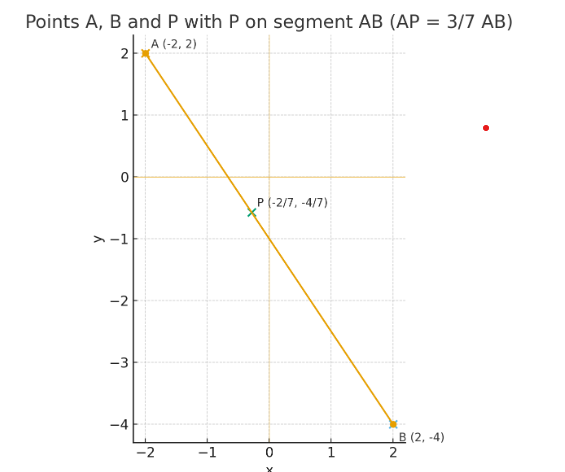
\includegraphics[width=0.6\columnwidth]{figs/fig1.png}
\end{center}
\end{frame}

\end{document}